% Pregunta 34 (2002-octubre-OEP2002): carteras de Markowitz en el plano (sigma_i, E_i).
% Redibujado del escaneo del examen. Autor: Víctor Gutiérrez Marcos
\documentclass[tikz,border=8pt]{standalone}
\usepackage[T1]{fontenc}
\usepackage{newpxtext,newpxmath}
\begin{document}
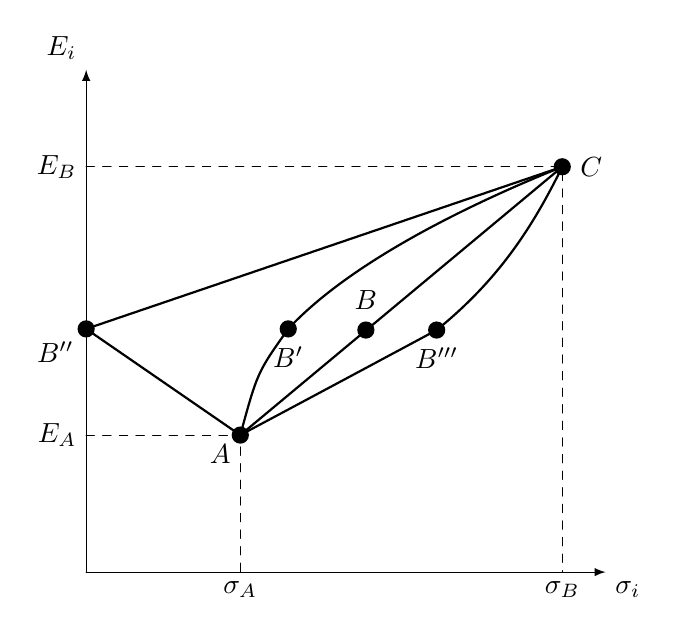
\begin{tikzpicture}[x=1.45cm,y=1.45cm,line cap=round,
    punto/.style={circle,fill=black,inner sep=2.2pt}]
  \coordinate (A) at (1.35,1.2);  \coordinate (C) at (4.17,3.55);
  \coordinate (B2) at (0,2.13);   \coordinate (B1) at (1.77,2.13);
  \coordinate (B) at (2.45,2.12); \coordinate (B3) at (3.07,2.12);
  \draw[->,>=latex] (0,0) -- (4.55,0) node[below right] {$\sigma_i$};
  \draw[->,>=latex] (0,0) -- (0,4.4) node[above left] {$E_i$};
  \draw[dashed] (0,1.2) node[left] {$E_A$} -- (A) -- (1.35,0) node[below] {$\sigma_A$};
  \draw[dashed] (0,3.55) node[left] {$E_B$} -- (C) -- (4.17,0) node[below] {$\sigma_B$};
  \draw[thick] (A) -- (B2) -- (C);
  \draw[thick] (A) -- (C);
  \draw[thick] (A) .. controls (1.5,1.75) .. (B1) .. controls (2.3,2.7) and (3.3,3.2) .. (C);
  \draw[thick] (A) .. controls (2.1,1.6) .. (B3) .. controls (3.6,2.55) and (3.9,3) .. (C);
  \foreach \p in {A,C,B2,B1,B,B3} \node[punto] at (\p) {};
  \node[below left] at (A) {$A$};
  \node[right=3pt] at (C) {$C$};
  \node[below left=1pt] at (B2) {$B''$};
  \node[below=3pt] at (B1) {$B'$};
  \node[above=4pt] at (B) {$B$};
  \node[below=3pt] at (B3) {$B'''$};
\end{tikzpicture}
\end{document}
